\documentclass[12pt]{beamer}
\let\Tiny=\tiny
\usetheme{Air}
\usepackage{wasysym}
% \usepackage{ucs}
\usepackage[utf8x]{inputenc}
\usepackage[ngerman]{babel}
\usepackage{verbatim}
\usepackage{listings}
\usepackage{multicol}

\pdfinfo
{
  /Title       (YWEE -- Personal Tutoring Service)
  /Creator     (TeX)
  /Author      (Daniel Tatzel)
}

\title{YWEE}
\subtitle{Personal Tutoring Service \\ Gruppe 2}
% \author{Nils Weiß \and \textbf{Daniel Tatzel} \and Alexander Strobl \\ \and Tobias Schwindl \and Florian Laufenböck \\ \and Matthias Birnthaler \and Matthias Götz \\ \and Maximilian Schröter}
\author{Weiß \and \textbf{ Daniel Tatzel} \and Strobl \and Schwindl \and Laufenböck  \and Birnthaler \and Schröter \and Götz}
\newcommand{\autor}{Daniel Tatzel}
\date{02. Juli 2014}

      \definecolor{dkgreen}{rgb}{0,.6,0}
      \definecolor{dkblue}{rgb}{0,0,.6}
      \definecolor{dkyellow}{cmyk}{0,0,.8,.3}

      %%%%%%%%%%%%%%%%%%% JAVA SCRIPT SUPPORT %%%%%%%%%%%%%%%%%%%%%%%%
\definecolor{lightgray}{rgb}{.9, .9, .9}
\definecolor{darkgray}{rgb}{.4, .4, .4}
\definecolor{purple}{rgb}{0.65, 0.12, 0.82}

\lstdefinelanguage{JavaScript}{
        keywords={typeof, new, true, false, catch, function, return, null, catch, switch, var, if, in, while, do, else, case, break},
        keywordstyle=\color{blue}\bfseries,
        ndkeywords={class, export, boolean, throw, implements, import, this},
        ndkeywordstyle=\color{darkgray}\bfseries,
        identifierstyle=\color{black},
        sensitive=false,
        comment=[l]{//},
        morecomment=[s]{/*}{*/},
        commentstyle=\color{purple}\ttfamily,
        stringstyle=\color{red}\ttfamily,
        morestring=[b]',
        morestring=[b]"
        }

\begin{document}

\frame{\titlepage}

\section*{}
\begin{frame}
  \frametitle{Agenda}
  \tableofcontents[hidesubsections]
\end{frame}

\AtBeginSection[]
{
  \frame<handout:0>
  {
    \frametitle{Agenda}
    \tableofcontents[currentsection, currentsubsection, sectionstyle=show/shaded, subsectionstyle=show/show/hide, subsubsectionstyle=show/show]
  }
}

\newcommand<>{\highlighton}[1]{%
  \alt#2{\structure{#1}}{{#1}}
}

\newcommand{\icon}[1]{\pgfimage[height=1em]{#1}}

\newcommand{\phpcode}{
      \lstset{
	language        = php,
	backgroundcolor=\color{lightgray},
	extendedchars=true,
	basicstyle=\tiny\ttfamily,
	showstringspaces=false,
	showspaces=false,
	numbers=left,
	numberstyle=\tiny\ttfamily,
	numbersep=9pt,
	tabsize=2,
	breaklines=true,
	showtabs=false,
	frame=leftline,
	keywordstyle    = \color{dkblue},
	stringstyle     = \color{red},
	identifierstyle = \color{dkgreen},
	commentstyle    = \color{gray},
	emph            =[1]{php},
	emphstyle       =[1]\color{black},
	emph            =[2]{if,and,or,else},
	emphstyle       =[2]\color{dkyellow}
	}
  }

  \newcommand{\jscode}{
      \lstset{
        language=JavaScript,
        backgroundcolor=\color{lightgray},
        extendedchars=true,
        basicstyle=\tiny\ttfamily,
        showstringspaces=false,
        showspaces=false,
        numbers=left,
        numberstyle=\tiny\ttfamily,
        numbersep=9pt,
        tabsize=2,
        breaklines=true,
        showtabs=false,
        frame=leftline,
        literate={\$}{{\textcolor{blue}{\$}}}1,
        mathescape=false
        }
  }

%%%%%%%%%%%%%%%%%%%%%%%%%%%%%%%%%%%%%%%%%
%%%%%%%%%% YWEE content starts here %%%%%%%%%%
%%%%%%%%%%%%%%%%%%%%%%%%%%%%%%%%%%%%%%%%%
% Einleitung
\section{Aufgaben} % "Sowas wie Kapitel"
%\subsection{Aufgaben} % Unter Kapitel

\begin{frame} %%Eine Folie
%   \frametitle{Tutoren Agentur} %%Folientitel
% Definitionsblock
	Im Team Backend mit Florian Laufenböck und Daniel Tatzel
	
	Zuständig für:
	\begin{itemize}
	\item Nachrichten
	\item Spende
	\item Autocomplete in der Suche
	\end{itemize}
\end{frame}


% SRA
\include{./chapters/2_SRA}

% SAD
\include{./chapters/3_SAD}

% Implementierung
\section{Implementierung}
\subsection{Code}
\defverbatim[colored]
  \makeset{
    \phpcode

      \begin{lstlisting}[name=upload.php]
<?php
/* Passwortaenderung fuer den Privaten Ordner -- Daniel Tatzel */

/* create_htpasswd: Generiert eine .htpasswd Datei mit Benutzername und Passwort fuer den Login zum Privaten Ordner */
    $DIR = $_SERVER["DOCUMENT_ROOT"] . "/test_02/private/";
    if ( file_exists($DIR . '.htpasswd') )
        unlink($DIR.'.htpasswd');

    $passwd = crypt($_POST['passwd']);
    $htpasswd = 'admin:' . $passwd . "\n";

    $stream = "# Autor: Daniel Tatzel\n\n".$htpasswd;

    $handle = fopen($DIR . '.htpasswd',"a");
    fputs($handle,$stream);
    fclose($handle);

    header("Location: http://www.ebenezer-kunatse.net/private/");
?>
      \end{lstlisting}
}

\begin{frame}
  \frametitle{Passwort ändern}
  \makeset
\end{frame}

\defverbatim[colored]
  \makeset{
    \phpcode

      \begin{lstlisting}[name=ListDir.php]
<?php
    // Autor von ListDir.php: Daniel Tatzel
    // Liest alle Dateien aus, berechnet die Groesse in KB und erzeugt ein JSON objekt

    $Dir = "./files/";	// Zielordner

    // Kann dann mit JSON in Javascript umgewandelt werden zur Verarbeitung ( Array )
    $FileListing = array_diff(scandir($Dir), array('..', '.'));

    // Wird nur ausgefuehrt falls Daten vorhanden sind
    if ( count( $FileListing ) > 0 )
    {
        $file_arr = array();

        foreach ( $FileListing as $File )
        {
            $size = number_format( filesize($Dir.$File)/1024, 2, ",", "." );

            // Array fuer JSON Objekt
            $file_arr[] = array("name" => $File, "size" => $size);
        }

        echo json_encode( $file_arr );	// JSON Ausgabe
    }
?>
      \end{lstlisting}
  }

\begin{frame}
  \frametitle{Verzeichnis Inhalt holen}
  \makeset
\end{frame}

\defverbatim[colored]
  \makeset{
    \phpcode

      \begin{lstlisting}[name=upload.php]
<?php
    // Autor von upload.php: Daniel Tatzel
    // Laedt eine ausgewaehlte Datei auf den Server hoch

    $temp = explode(".", $_FILES["file"]["name"]);
    $extension = end($temp);

    // Gibt eine Meldung aus, falls ein Fehler aufgetreten ist
    if ($_FILES["file"]["error"] > 0)
    {
        echo "Fehler Code: " . $_FILES["file"]["error"] . "<br>";
    }
    else
    {
        // Prueft ob Datei schon vorhanden ist und gibt eine Meldung aus, ansonsten wird die Datei hochgeladen
        if (file_exists($_SERVER["DOCUMENT_ROOT"] . "/test_02/private/files/" . $_FILES["file"]["name"])) {
          echo $_FILES["file"]["name"] . " bereits vorhanden. ";
        }
        else {
          move_uploaded_file($_FILES["file"]["tmp_name"],
          $_SERVER["DOCUMENT_ROOT"] . "/test_02/private/files/" . $_FILES["file"]["name"]);
        }
    }
?>

      \end{lstlisting}
  }

\begin{frame}
  \frametitle{Datei hochladen}
  \makeset
\end{frame}

\defverbatim[colored]
  \makeset{
    \jscode

      \begin{lstlisting}[name=hide.js]
<script language="javascript">
    function show(selector)
    {
        var sel = selector;

        if ( sel == 0 )
            sel = "passwd";
        else
            sel = "file"

        if(document.getElementById( sel ).style.display == 'block')
        {
            document.getElementById( sel ).style.display = 'none';
        }
        else
        {
            document.getElementById( sel ).style.display = 'block';
        }
    }
</script>
      \end{lstlisting}
  }

\begin{frame}
  \frametitle{Ausblenden von Bereichen}
  \makeset
\end{frame}

\defverbatim[colored]
  \makeset{
    \jscode

      \begin{lstlisting}[name=table.js]
$(document).ready(function() {
    var mTable = $('#filesTable').dataTable({
        "oLanguage": {
            "sSearch": "Dateien filtern:",
            "oPaginate": {
                "sNext": "Naechste Seite",
                "sPrevious": "Vorherige Seite"
            },
            "sInfo": "Es wurden _TOTAL_ Dateien gefunden. Aktuelle Anzeige (_START_ bis _END_)",
            "sLengthMenu": "Zeige _MENU_ Dateien"
        }
    });
    mTable.fnClearTable();
    jQuery.each(files, function() {
        mTable.fnAddData(['<a href="files/' + this.name + '" > ' + this.name + '</a>', this.size, '<form method="POST" action=""><input type="hidden" name="file" value="'+ this.name +'"><input type="submit" name="delete" value="L&ouml;schen"></form>']);
    });
    mTable.draw();
  });
      \end{lstlisting}
  }

\begin{frame}
  \frametitle{Erstellen der Tabelle}
  \makeset
\end{frame}

\defverbatim[colored]
  \makeset{
    \phpcode

      \begin{lstlisting}[name=delete.php]
<?php
    // Autor von delete.php: Daniel Tatzel
    // Loescht eine Datei

    $path = realpath('files/'.$_POST['file']);

    // Wenn vorhanden, dann l&oeschen
    if( is_file($path) )
        unlink( $path );
?>
      \end{lstlisting}
  }

\begin{frame}
  \frametitle{Löschen einer Datei}
  \makeset
\end{frame}

\subsection{Screenshot}
\begin{frame}
  \frametitle{Screenshot}
  \begin{figure}[htbp]
    \centering
    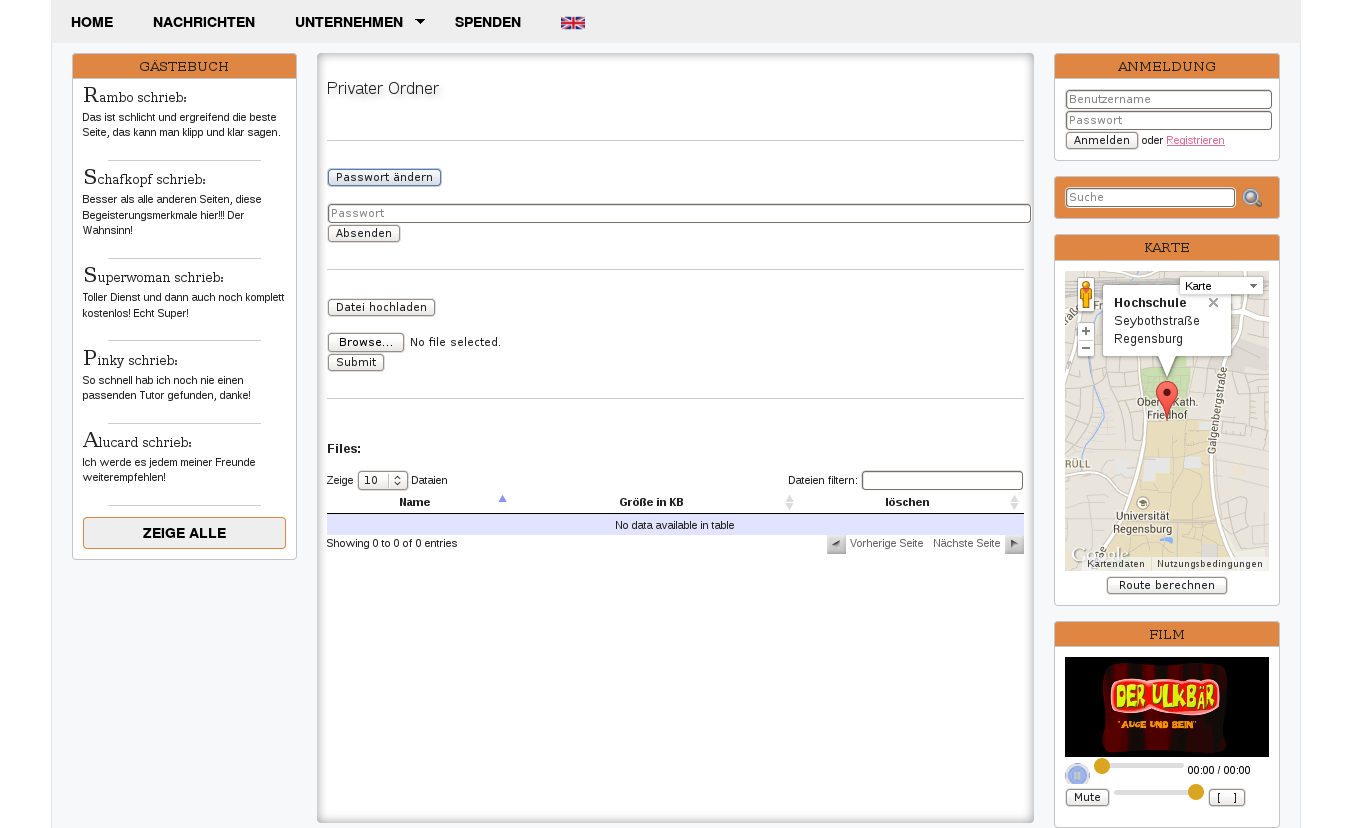
\includegraphics[width=1.0\textwidth]{./chapters/privdir}
    \caption{Ansicht des Privaten Ordners}
    \label{fig:privdir}
  \end{figure}
\end{frame}

\subsection{Demonstration}
\begin{frame} %%Eine Folie
  \frametitle{Demonstration} %%Folientitel

% Fettgedruckt
  \center
  \textbf{Es folgt eine Demonstration ...}
\end{frame}

%%%%%%%%%%%%%%%%%%%%%%%%%%%%%%%%%%%%%%%%%
%%%%%%%%%%%%%%%%%%%%%%%%%%%%%%%%%%%%%%%%%
%%%%%%%%%% Latex Tutorial Content starts here %%%%%%%%%%
%%%%%%%%%%%%%%%%%%%%%%%%%%%%%%%%%%%%%%%%%

\end{document}
